%%%%%%%%%%%%%%%%%%%%%%%%%%%%%%%%%%%%%%%%%
% Jacobs Landscape Poster
% LaTeX Template
% Version 1.0 (29/03/13)
%
% Created by:
% Computational Physics and Biophysics Group, Jacobs University
% https://teamwork.jacobs-university.de:8443/confluence/display/CoPandBiG/LaTeX+Poster
%
% Further modified by:
% Nathaniel Johnston (nathaniel@njohnston.ca)
%
% This template has been downloaded from:
% http://www.LaTeXTemplates.com
%
% License:
% CC BY-NC-SA 3.0 (http://creativecommons.org/licenses/by-nc-sa/3.0/)
%
%%%%%%%%%%%%%%%%%%%%%%%%%%%%%%%%%%%%%%%%%

%----------------------------------------------------------------------------------------
%	PACKAGES AND OTHER DOCUMENT CONFIGURATIONS
%----------------------------------------------------------------------------------------

\documentclass[final]{beamer}

\usepackage[scale=0.8,size=a1]{beamerposter} % Use the beamerposter package for laying out the poster

\usetheme{confposter} % Use the confposter theme supplied with this template

\setbeamercolor{block title}{fg=ngreen,bg=white} % Colors of the block titles
\setbeamercolor{block body}{fg=black,bg=white} % Colors of the body of blocks
\setbeamercolor{block alerted title}{fg=white,bg=dblue!70} % Colors of the highlighted block titles
\setbeamercolor{block alerted body}{fg=black,bg=dblue!10} % Colors of the body of highlighted blocks
% Many more colors are available for use in beamerthemeconfposter.sty

%-----------------------------------------------------------
% Define the column widths and overall poster size
% To set effective sepwid, onecolwid and twocolwid values, first choose how many columns you want and how much separation you want between columns
% In this template, the separation width chosen is 0.024 of the paper width and a 4-column layout
% onecolwid should therefore be (1-(# of columns+1)*sepwid)/# of columns e.g. (1-(4+1)*0.024)/4 = 0.22
% Set twocolwid to be (2*onecolwid)+sepwid = 0.464
% Set threecolwid to be (3*onecolwid)+2*sepwid = 0.708

\newlength{\sepwid}
\newlength{\onecolwid}
\newlength{\twocolwid}
\newlength{\threecolwid}
\setlength{\paperwidth}{36in} % A0 width: 46.8in
\setlength{\paperheight}{24in} % A0 height: 33.1in
\setlength{\sepwid}{0.024\paperwidth} % Separation width (white space) between columns
\setlength{\onecolwid}{0.218\paperwidth} % Width of one column
\setlength{\twocolwid}{0.464\paperwidth} % Width of two columns
\setlength{\threecolwid}{0.708\paperwidth} % Width of three columns
\setlength{\topmargin}{-0.5in} % Reduce the top margin size
\usepackage{graphicx}  % Required for including images
\usepackage{booktabs} % Top and bottom rules for tables

%----------------------------------------------------------------------------------------
%	TITLE SECTION
%----------------------------------------------------------------------------------------

\title{Web service for 19\textsuperscript{th} century Irish personal name matching} % Poster title

\author{Phattara Wangrungarun and Dr Adam Winstanley (supervisor)} % Author(s)

\institute{Erasmus Mundus -- MSc in Dependable Software Systems (DESEM) -- Maynooth University -- 2014/15} % Institution(s)

%----------------------------------------------------------------------------------------

\begin{document}

\addtobeamertemplate{block end}{}{\vspace*{2ex}} % White space under blocks
\addtobeamertemplate{block alerted end}{}{\vspace*{2ex}} % White space under highlighted (alert) blocks

\setlength{\belowcaptionskip}{2ex} % White space under figures
\setlength\belowdisplayshortskip{2ex} % White space under equations

\begin{frame}[t] % The whole poster is enclosed in one beamer frame

\begin{columns}[t] % The whole poster consists of three major columns, the second of which is split into two columns twice - the [t] option aligns each column's content to the top

\begin{column}{\sepwid}\end{column} % Empty spacer column

\begin{column}{\onecolwid} % The first column

\begin{block}{Abstract}

Before the first Irish civil registration on 1864, census materials
were mostly lost or incomplete. So genealogical research uses
parish records and also some `census substitute' documents,
such as land ownership and tenancy records. However, some of these documents
may not contain enough information in identify individuals.
Some of them contains a name and address,
whereas others might contain only a name.

\emph{Record linkage} is one method to gather scattered information among many documents.
It uses a person\textquotesingle s name as a reference to link that
person\textquotesingle s information between many documents. With patience,
a more complete information about that person can be obtained.

Therefore linking or matching a person\textquotesingle s name is important in the process.
Unfortunately, in the 19\textsuperscript{th} century, in Ireland, there was no standard
spelling of names, handwriting could be difficult to read
and contractions or abbreviations were often used. The names with the same
pronunciation and for the same individual could be written in many different ways.
Moreover, names in the Irish language which are equivalent to English names
were used, for example, Irish version of `Smith' could be `Gowan'.
A further complication is that historical  and genealogical research often
requires large quantities of names to be matched.

To handle these name variations, various solutions have been created to find
matching different names that refer to the same person. However,
for our extent knowledge, there is yet no public system which encodes
those solutions together and provides a service of bulk name matching.

Thus, we developed a web service system using Ruby on Rails framework
to achieve our goal. The system is initially encoded with 4 matching algorithms,
Levenshtein distance, soundex, Irish soundex, and lookup table.

% We also present a web interface for a client to use the system
% from the web browser. It is designed to be simple and extensible from using
% inheritance.

% The system performs matchings on large quantities of names in a reasonable time.
% We test our system with 12,944 name matchings and the result were completed
% in no more than half a minute (28,786 milliseconds, to be precise).
% However, the system consumes a large amount of memory (around 373 megabytes).
% We believe that, with proper optimisation, we would reduce the memory usage
% along with a shortened processing time. Further matching algorithms could also
% be implemented for names in other languages, so that it can handle
% a broader domain of names.

\end{block}

\begin{alertblock}{Research Questions}

\begin{itemize}
\item Can we provide a web service to match names, where matching can be
      a complicated process because of the way people record their names.
\item Can the web service act as a platform system for general names or words
      matching system so that it can be extended to other languages as well.
\end{itemize}

\end{alertblock}


\end{column}

\begin{column}{\sepwid}\end{column}

% \begin{column}{\onecolwid}
%
% \end{column}
%
% \begin{column}{\sepwid}\end{column}
%
% \begin{column}{\onecolwid}
%
% \begin{block}{Abtract}
%
% \end{block}
%
% \end{column}

\begin{column}{\twocolwid} % Begin a column which is two columns wide (column 2)

\begin{columns}[t,totalwidth=\twocolwid] % Split up the two columns wide column

\begin{column}{\onecolwid}\vspace{-.4in} % The first column within column 2 (column 2.1)

\begin{block}{Initial Idea}

\begin{figure}
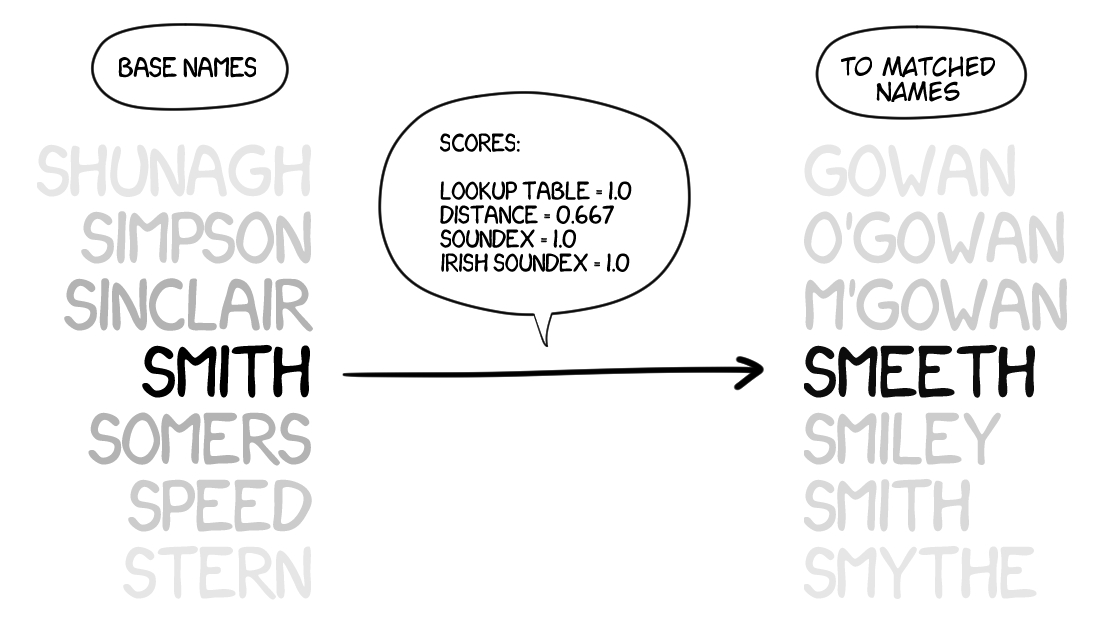
\includegraphics[width=1\linewidth]{gfx/base_tmn}
\end{figure}

\emph{Base name}
`SMITH' comparing to \emph{to-match name} `SMEETH'.
Scores of each matching algorithms
are presented in the bubble above the arrow.

\end{block}

\begin{block}{Actual System}
\begin{figure}
\makebox[\textwidth][c]{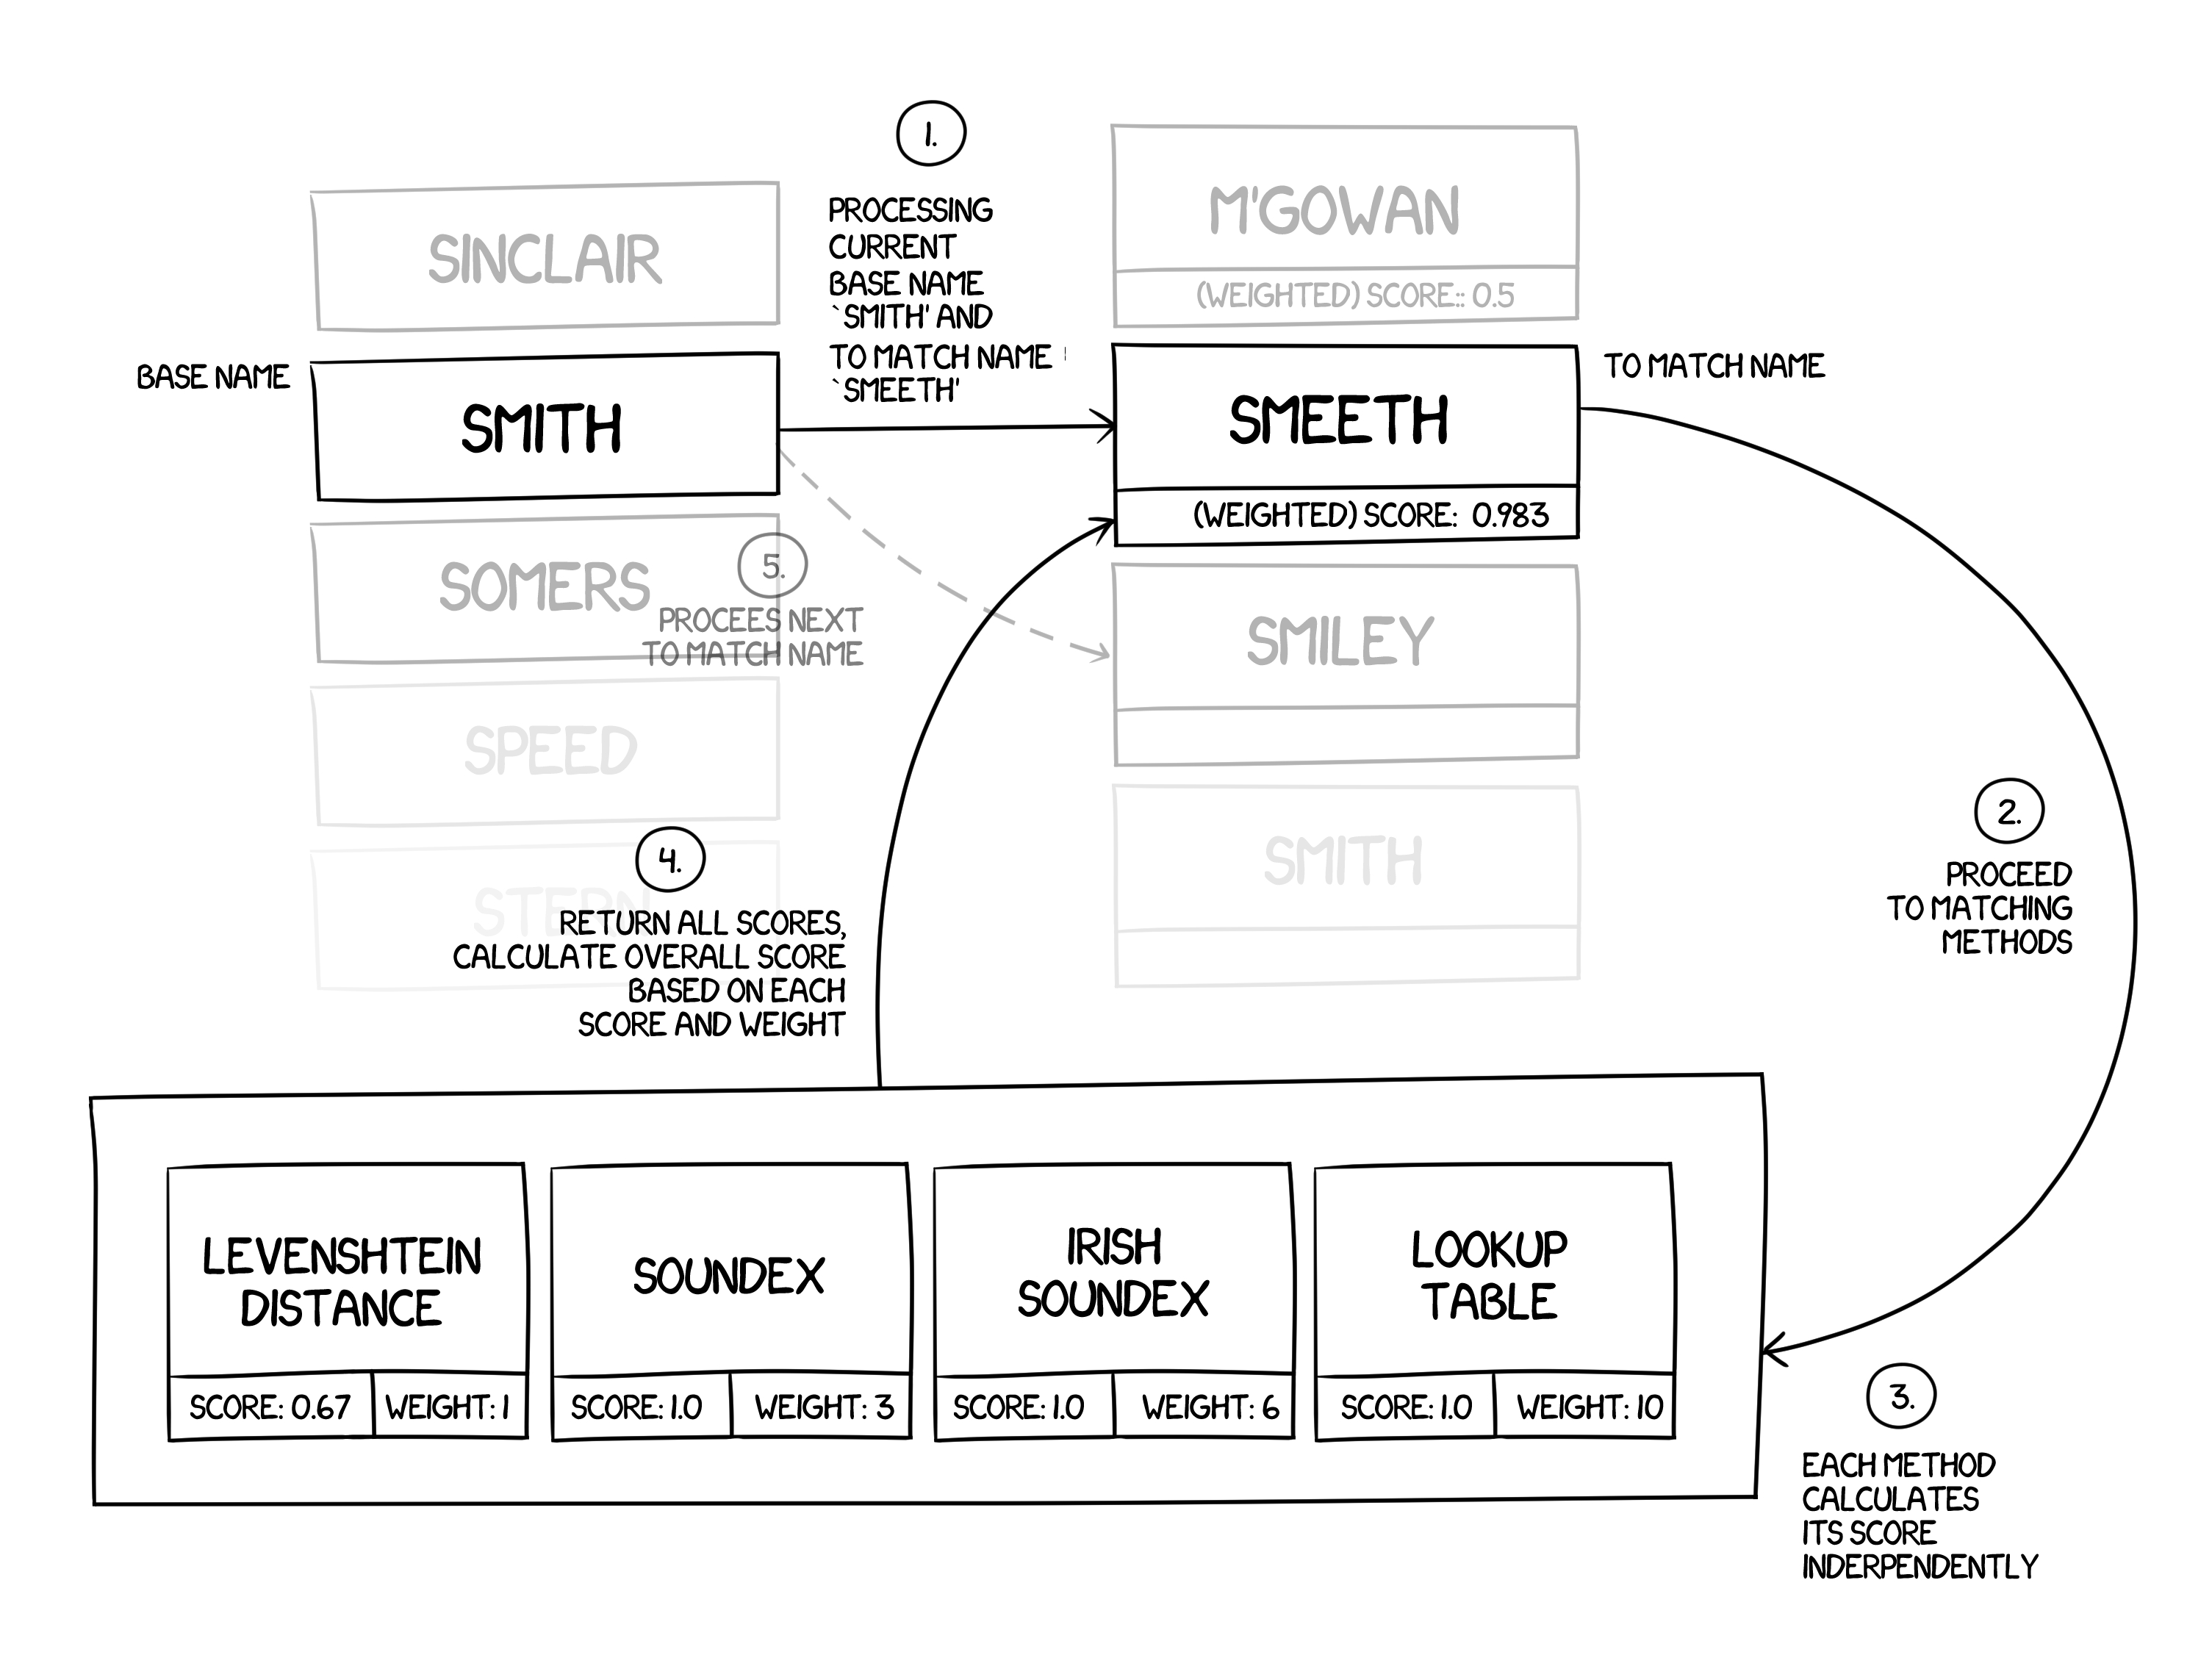
\includegraphics[width=1.1\linewidth]{gfx/overall}}
\end{figure}

One matching cycle consists of 5 steps.

\begin{enumerate}
  \item Processing current \emph{base name} `SMITH' and \emph{to-match name} `SMEETH'
  \item Proceed to matching algorithms.
  \item Each algorithm calculates its score indepedently.
  \item Calculate \emph{overall weighted score}.
  \item Matching cycle for `SMITH' and `SMEETH' is finished with
    \emph{overall weighted score} 0.983.
\end{enumerate}

\end{block}

\end{column} % End of column 2.1

\begin{column}{\onecolwid}\vspace{-.4in} % The second column within column 2 (column 2.2)

\begin{block}{MVC}

\begin{figure}
\makebox[\textwidth][c]{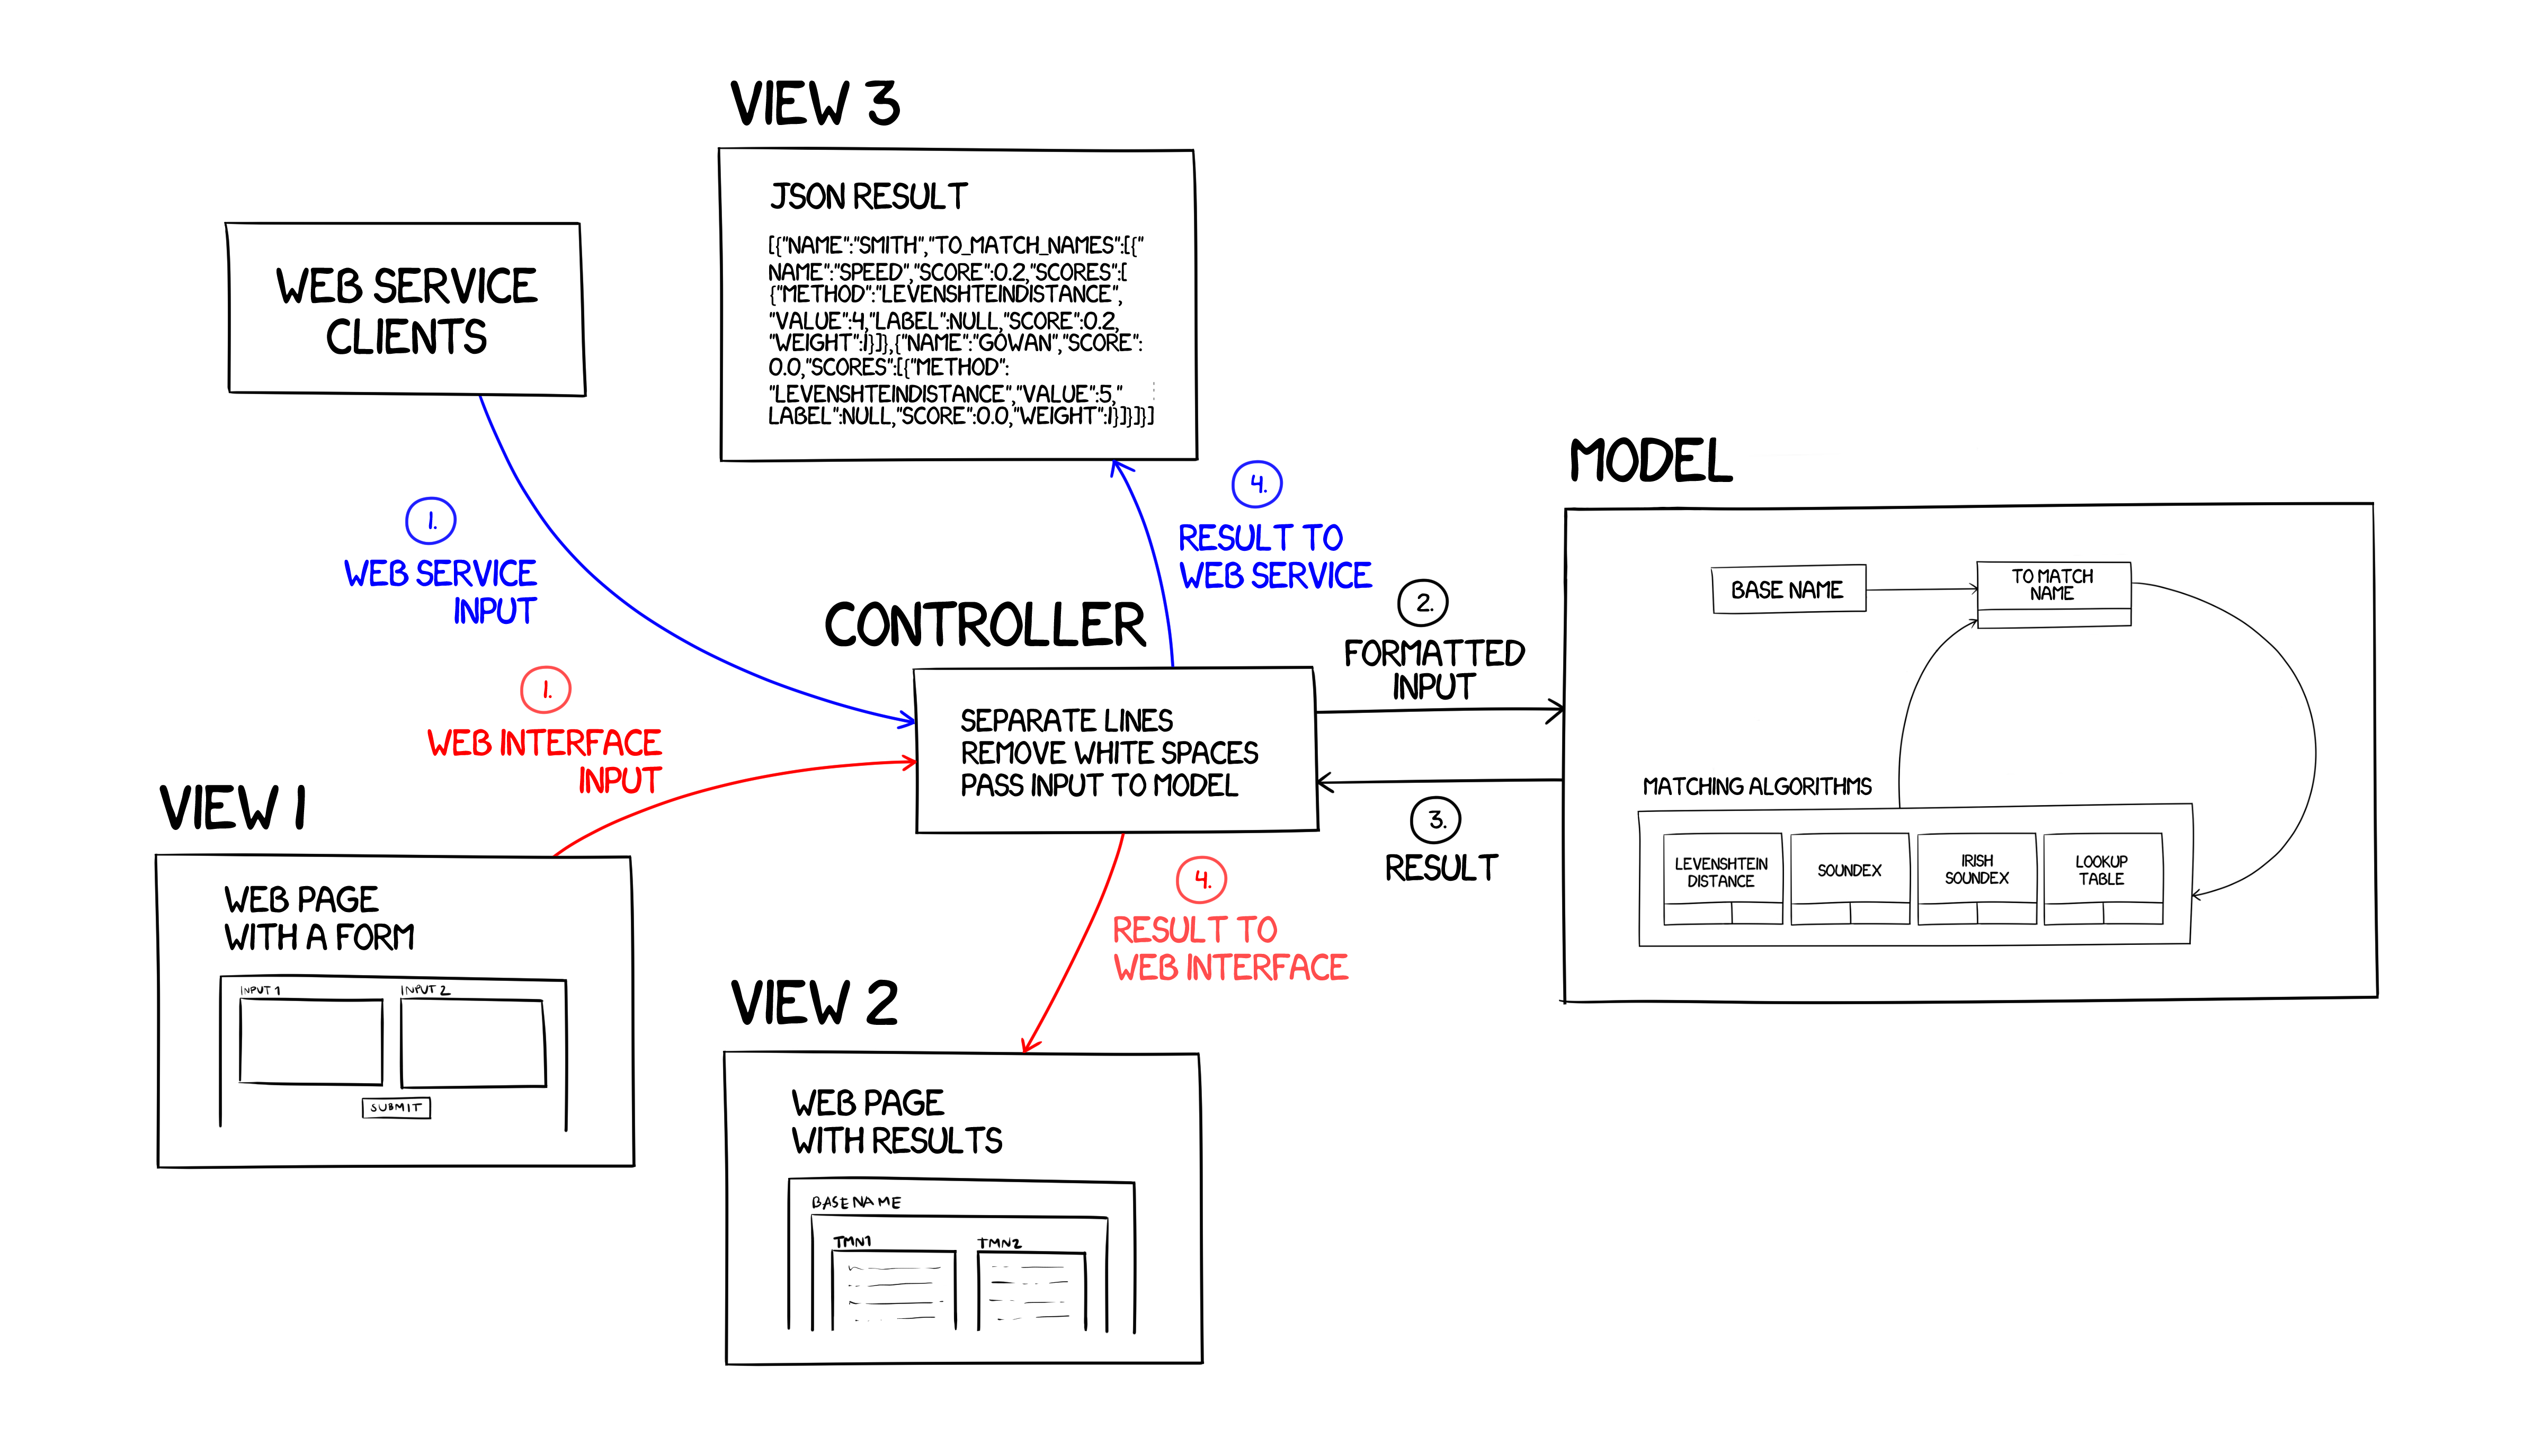
\includegraphics[width=1.1\linewidth]{gfx/mvc}}
\end{figure}

\end{block}

\begin{block}{Web Service}

% Here is an attempt to match between base name `SMITH',
% and to-match name `SMYTHE' and `O'GOWAN'. Using 4 matching algorithms,
% and threshold as 0. We will submit this sample.json input to the system
% using cURL in command line.
% We use HTTP POST to submit to the web service.
% The formatted JSON result is shown below,
% note that the result is truncated just for readability.

\begin{figure}
\makebox[\textwidth][c]{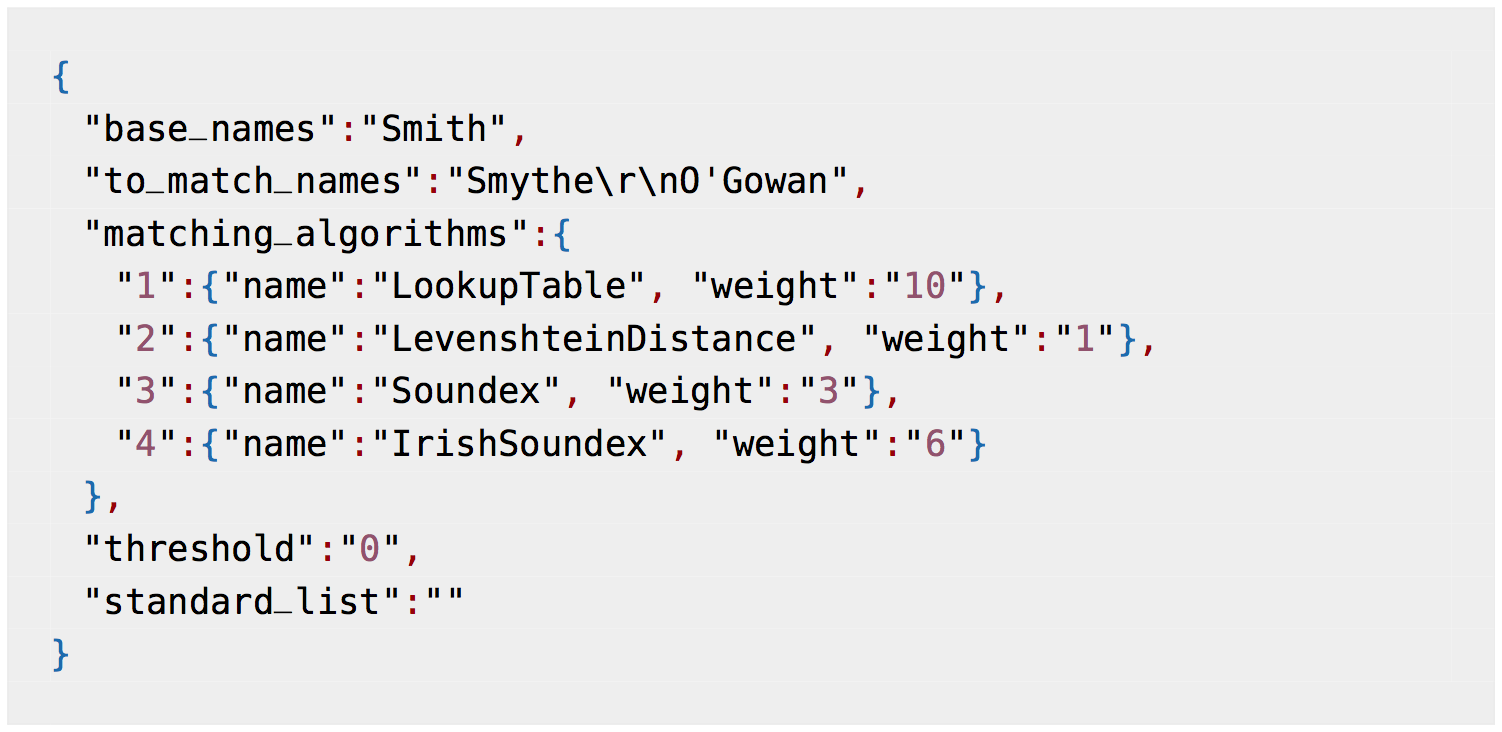
\includegraphics[width=0.8\linewidth]{gfx/p1}}
\end{figure}
\begin{figure}

\makebox[\textwidth][c]{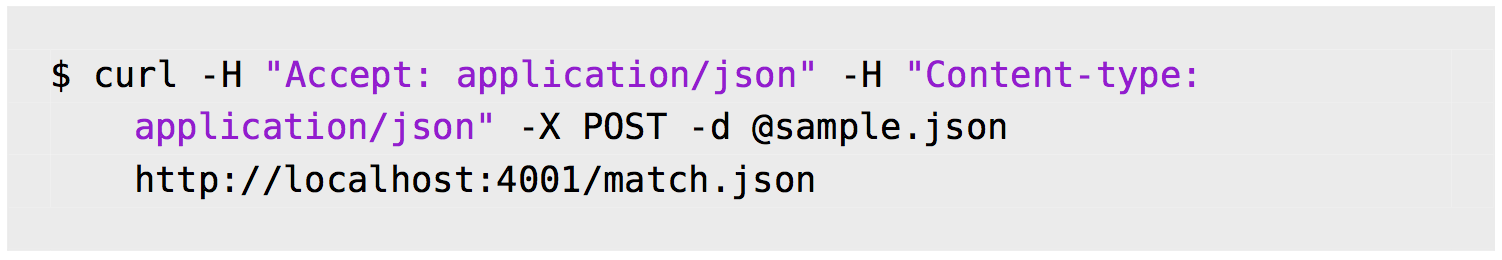
\includegraphics[width=0.8\linewidth]{gfx/p2}}
\end{figure}
\begin{figure}

\makebox[\textwidth][c]{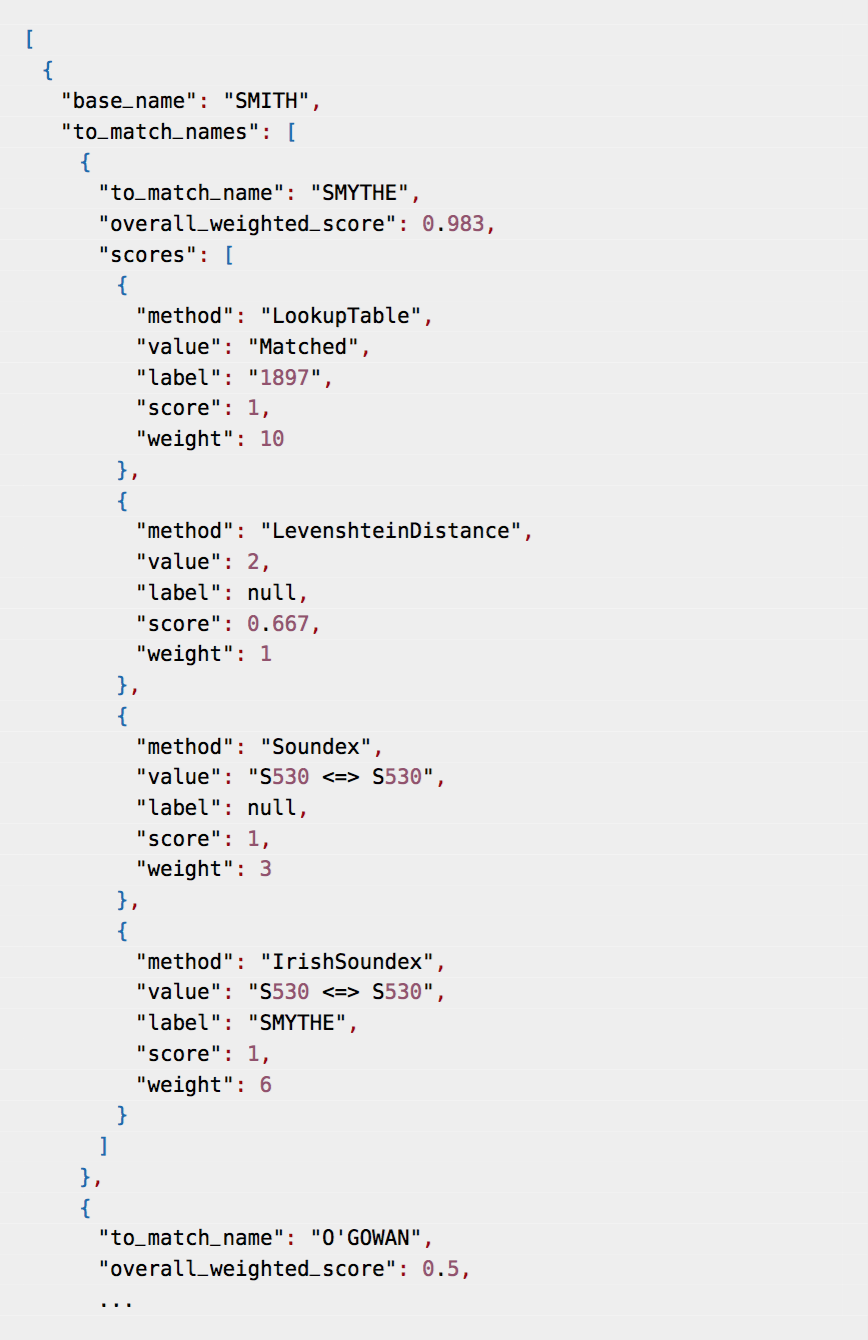
\includegraphics[width=0.53\linewidth]{gfx/p3}}
\end{figure}
\end{block}

\end{column} % End of column 2.2

\end{columns} % End of the split of column 2 - any content after this will now take up 2 columns width

% \begin{columns}[t,totalwidth=\twocolwid] % Split up the two columns wide column again
%
% \begin{column}{\onecolwid} % The first column within column 2 (column 2.1)
%
% \begin{block}{Mathematical Section}
%
% Nam quis odio enim, in molestie libero. Vivamus cursus mi at nulla elementum sollicitudin. Nam quis odio enim, in molestie libero. Vivamus cursus mi at nulla elementum sollicitudin.
%
% \begin{equation}
% E = mc^{2}
% \label{eqn:Einstein}
% \end{equation}
%
% Nam quis odio enim, in molestie libero. Vivamus cursus mi at nulla elementum sollicitudin. Nam quis odio enim, in molestie libero. Vivamus cursus mi at nulla elementum sollicitudin.
%
% \begin{equation}
% \cos^3 \theta =\frac{1}{4}\cos\theta+\frac{3}{4}\cos 3\theta
% \label{eq:refname}
% \end{equation}
%
% Nam quis odio enim, in molestie libero. Vivamus cursus mi at nulla elementum sollicitudin. Nam quis odio enim, in molestie libero. Vivamus cursus mi at nulla elementum sollicitudin.
%
% \begin{equation}
% \kappa =\frac{\xi}{E_{\mathrm{max}}} %\mathbb{ZNR}
% \end{equation}
%
% \end{block}
%
% \end{column} % End of column 2.1
%
% \begin{column}{\onecolwid} % The second column within column 2 (column 2.2)
%
% \begin{block}{Results}
%
% \begin{figure}
% 
\includegraphics[width=0.8\linewidth]{placeholder.jpg}
% \caption{Figure caption}
% \end{figure}
%
% Nunc tempus venenatis facilisis. Curabitur suscipit consequat eros non porttitor. Sed a massa dolor, id ornare enim:
%
% \begin{table}
% \vspace{2ex}
% \begin{tabular}{l l l}
% \toprule
% \textbf{Treatments} & \textbf{Response 1} & \textbf{Response 2}\\
% \midrule
% Treatment 1 & 0.0003262 & 0.562 \\
% Treatment 2 & 0.0015681 & 0.910 \\
% Treatment 3 & 0.0009271 & 0.296 \\
% \bottomrule
% \end{tabular}
% \caption{Table caption}
% \end{table}
%
% \end{block}
%
% \end{column} % End of column 2.2
%
% \end{columns} % End of the split of column 2

\end{column} % End of the second column

\begin{column}{\sepwid}\end{column} % Empty spacer column

\begin{column}{\onecolwid} % The third column

\begin{block}{Evaluation}

We tested our system by matching 12,944 names.

\begin{table}
\vspace{2ex}
\begin{tabular}{l l }
\toprule
\textbf{Matching algorithms} & \textbf{Response speed (ms)}\\
\midrule
Levenshtein distance & 1,337 \\
Soundex & 2,024 \\
Irish soundex & 2,456 \\
Lookup table & 24,293 \\
\midrule
All 4 algorithms & 28,786 \\
\bottomrule
\end{tabular}
\caption{Response speed for each matching algorithms.}
\end{table}
\begin{table}
\vspace{2ex}
\begin{tabular}{l l }
\toprule
\textbf{Matching algorithms} & \textbf{Memory usage (bytes)}\\
\midrule
Levenshtein distance & 48,518,621 \\
Soundex & 53,066,150 \\
Irish soundex & 69,534,598 \\
Lookup table & 244,302,744 \\
\midrule
All 4 algorithms & 373,544,727 \\
\bottomrule
\end{tabular}
\caption{Memory usage for each matching algorithms.}
\end{table}
\end{block}

\begin{block}{References}

\nocite{*} % Insert publications even if they are not cited in the poster
\small{\bibliographystyle{unsrt}
\bibliography{sample}\vspace{0.75in}}

\end{block}

% \setbeamercolor{block title}{fg=red,bg=white} % Change the block title color
%
% \begin{block}{Acknowledgements}
%
% \small{\rmfamily{Nam mollis tristique neque eu luctus. Suspendisse rutrum congue nisi sed convallis. Aenean id neque dolor. Pellentesque habitant morbi tristique senectus et netus et malesuada fames ac turpis egestas.}} \\
%
% \end{block}

\setbeamercolor{block alerted title}{fg=black,bg=norange} % Change the alert block title colors
\setbeamercolor{block alerted body}{fg=black,bg=white} % Change the alert block body colors

% \begin{alertblock}{Contact Information}
%
% \begin{itemize}
% \item Web: \href{http://www.university.edu/smithlab}{http://www.university.edu/smithlab}
% \item Email: \href{mailto:john@smith.com}{john@smith.com}
% \item Phone: +1 (000) 111 1111
% \end{itemize}
%
% \end{alertblock}

\begin{center}
\begin{tabular}{ccc}

\includegraphics[height=0.25\linewidth]{gfx/mu} & \hfill & 
\includegraphics[height=0.25\linewidth]{gfx/em}
\end{tabular}
\end{center}

%----------------------------------------------------------------------------------------

\end{column} % End of the third column

\end{columns} % End of all the columns in the poster

\end{frame} % End of the enclosing frame

\end{document}
